\documentclass{article}
\usepackage{algorithm}
\usepackage{algpseudocode}
\usepackage{svg}
\usepackage{xcolor}
\usepackage{float}
\usepackage{amsmath,amsthm}
\usepackage{amsfonts}
\usepackage{graphicx}
\usepackage{pdfpages}
\usepackage{mathtools}
\bibliographystyle{plain}
\date{}

\theoremstyle{definition}
\newtheorem{definition}{Definition}[section]

\begin{document}
%\maketitle
%\thispagestyle{empty}
\section{Preliminaries}
Let $\mathbb{F}_2$ be the field of two elements, $\{0,1\}$. A polynomial ring, $\mathbb{F}_2[x_1,\dots,x_d]$, is the set of all polynomials in variables, $x_1,x_2,\dots,x_d$, and coefficients in the field $\mathbb{F}_2$. A monomial, $M = {x_1}^{\alpha_1}\cdots \allowbreak {x_d}^{\alpha_d}$, is a power product in the variables $x_1,\dots,x_d$ with $\alpha_i \geq 0$. A polynomial, $P \in \mathbb{F}[x_1,x_2,\dots,x_d]$, can be written as $P = c_1X_1 + c_2X_2 + \dots + c_tX_t$, where $c_1,\dots, c_t$ are the coefficients and $X_1, \dots, X_t$ are monomials. In this paper, the terms will be ordered lexicographically (LEX). 
\theoremstyle{definition}
\begin{definition}{{Boolean Polynomials~\cite{polybori}:}}
Let $P \in \mathbb{F}_2[x_1,x_2,\dots,x_d]/\langle {x_i}^2 - x_i\rangle$ be a Boolean polynomial, such that
\begin{center}
$P = c_1\cdot {x_1}^{\alpha_{11}}\cdots {x_d}^{\alpha_{1d}} + \cdots + c_t\cdot {x_t}^{\alpha_{t1}}\cdots {x_d}^{\alpha_{td}}$
\end{center} 
where, $c_i \in \mathbb{F}_2$ and $\alpha_{ij} \in \{0,1\}$.
\end{definition}
 
\begin{figure}
\centering
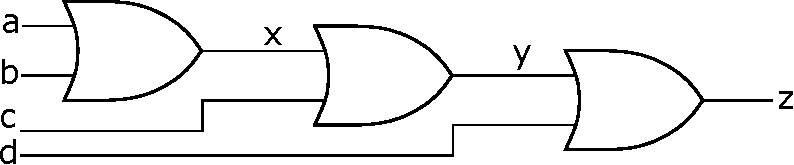
\includegraphics[scale=0.60]{Chain_Or_Gates.pdf}
\caption{A chain of OR gates}
\label{ChainOrGate}
\end{figure}
%\par Boolean Polynomials are the polynomials that belong to the quotient ring, $\mathbb{Z}_2[x_1,x_2,\dots,x_d]/\langle {x_i}^2 - x_i\rangle$, where $\mathbb{Z}_2$ is the set $\{0,1\}$. In other words, Boolean polynomials have coefficients either 0 or 1, and have degree 1. 
\par
The circuit under consideration is modeled as a set of Boolean polynomials using the following one-to-one mapping:
\begin{center}
$\neg a\rightarrow a + 1 \pmod{2}$ \\
$a \wedge b \rightarrow a \cdot b \pmod{2}$ \\
$a \vee b \rightarrow a \cdot b + a+ b \pmod{2}$\\
$a \oplus b \rightarrow a+b \pmod{2}$\\
\end{center} 
where, $a,b \in \{0,1\}$.
\par
%The negative signs in the equation above can be replaced with a positve signs as -1 $mo$d 2 = 1 $mod$ 2.
\textbf{Ideals and Varieties}~\cite{lv}: An \textit{ideal} $J$ generated by polynomials, $P_1,\dots P_s \in \mathbb{F}_2[x_1, \dots, x_d]$ is:
\begin{center}
$J = \langle P_1 \dots P_s \rangle = \{\sum_{i=1}^{s} h_i\cdot P_i: h_i \in \mathbb{F}_2[x_1,\dots, x_d]\}$
\end{center}
The polynomials, $P_1,\dots,P_s$, form the basis or generators of the ideal $J$. 
\par 
Let $\textbf{a} = (a_1,\dots, a_d) \in \mathbb{F}_{2}^{d}$ be a point, and $P \in \mathbb{F}_2[x_1,\dots,x_d]$ be a polynomial. We say that $P$ vanishes on $\textbf{a}$ if $P(\textbf{a}) = 0$. 
\par
For an ideal $J =  \langle P_1 \dots P_s \rangle$, the \textit{variety} of $J$ over $\mathbb{F}_2$ is:
\begin{center}
$V(J) = \{\textbf{a} \in \mathbb{F}_{2}^{d} : \forall P \in J, P(\textbf{a}) = 0\}$
\end{center}
\par 
\textbf{Gr\"obner basis}~\cite{lv}: There can be many different generators of an ideal $J$ i.e. $J = \langle P_1 \dots P_s \rangle = \langle Q_1 \dots Q_s \rangle$, where $\{P_1 \dots P_s\}$ and $\{Q_1 \dots Q_s\}$ are two different sets of polynomials. Gr\"obner basis is a particular kind of generating set of an ideal which allows to solve many polynomial decision problems. 
\par
The famous Buchberger's algorithm~\cite{Buchberger:1976} can compute the Gr\"obner basis of an ideal but at a very expensive computational complexity. 
A term order, called Reverse Topological Term Order (RTTO), derived from the topology of the circuit has been presented in~\cite{lv}. The polynomials for each gate with this order have the representation of the type, $P_i = x_i + tail(P_i)$. For example, the circuit in Figure~\ref{ChainOrGate} can have a variable ordering as, $z > f > e>d>c>b>a$. The polynomials for the three OR gates will be $P_1 = z + f\cdot d + f +d, P_2 = f + e\cdot c + e +c , P_3 = e + b\cdot a + b + a$. As the output of each gate is unique, the leading terms of all the polynomials corresponding to the circuit become relatively prime. Therefore, the RTTO obviates the need for computing a Grobner basis for this set of polynomials as this set is itself a Grobner basis. This term order is used in this paper hereafter.

%\subsection{Polynomial Reduction}
\par
\textbf{Polynomial Reduction:} Reduction of a polynomial $F$ $w.r.t.$ another polynomial $G$ is defined as follows:
\begin{equation}
F \xrightarrow{G} F - \frac{lt(F)}{lt(G)} \cdot G = F + \frac{lt(F)}{lt(G)} \cdot G
\end{equation}
where $lt(F)$ and $lt(G)$ denote the leading terms of polynomials, $F$ and $G$, respectively. Note that $-$ can be replaced with $+$ as $-1 \pmod{2} = 1 \pmod{2}$. This equation holds only if $lt(G)$ divides $lt(F)$. As we are working with circuits and RTTO, the expression for $G$ will always be like, $G = x_i + tail(G)$. Therefore, $F$ will be completely reduced by $G$ when there is no term in $F$ that contains $x_i$ in it and is represented as $F \xrightarrow{G}_{+}$.
%As we are working on polynomials modulo 2, the coefficients in the polynomials are either 1 or 0. Therefore, the above expression can be written as,
%\begin{equation}
%F - \frac{lm(F)}{lm(G)} \cdot G = F + \frac{lm(F)}{lm(G)} \cdot G
%\end{equation}
%where $lm(F)$ and $lm(G)$ denote the leading monomials of polynomials, $F$ and $G$, respectively. \\

\section{Theory}

Our verification procedure is based on reducing the output variables of the circuit $w.r.t$ the polynomials of the circuit which result in an expression composed of only input variables. This expression is canonical for a particular output. Next, we explain the reduction with an example and discuss how ZBDDs can improve the process.
\par
Consider, as an example, that we want to reduce the output, $F=z$, of the circuit in Figure~\ref{ChainOrGate} using Eqn. 1 (by $P_1, P_2, P_3$). The steps are:\\
\begin{enumerate}
\item $z \xrightarrow{P_1} f d +f +d$
\item $fd +f +d \xrightarrow{P_2} f + edc + ed + dc + d \xrightarrow{P_2} edc + ed + ec + e +dc + d + c$
\item $edc + ed + ec + e +dc + d + c \xrightarrow{P_3} ed + ec + e  + dcba  + dcb + dca + dc + d + c \xrightarrow{P_3} ec + e + dcba +dcb + dca + dc + dba + db + da + d + c \xrightarrow{P_3} e  +dcba +dcb + dca + dc + dba + db + da + d + cba + cb + ca + c \xrightarrow{P_3} dcba +dcb + dca + dc + dba + db + da + d + cba + cb + ca + c + ba + b +a$
\end{enumerate}
\begin{figure}
\centering
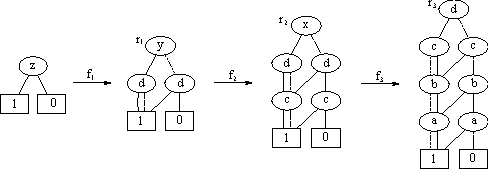
\includegraphics[scale=1.2]{red_steps.pdf}
\caption{Reduction of output of the circuit in Figure~\ref{ChainOrGate} by $P_1,P_2,P_3$}
\label{red_steps}
\end{figure}

%\begin{figure}
%\centering
%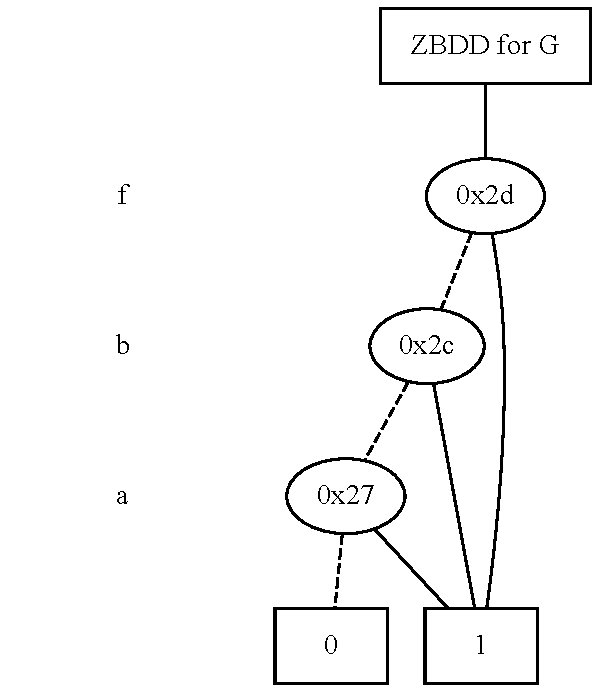
\includegraphics[scale=0.5]{fig2.pdf}
%\caption{Polynomial $G$}
%\label{G}
%\end{figure}

\par In the first step, $F$ is reduced by $P_1$ just once as there is only one term in $F$ that has $z$ in it. In the second step, the result of step one is reduced twice by $P_2$ as the result has two terms that have $f$ in them. Similarly, four reductions by $P_3$ are required to reduce the result of step two into an expression containing only primary inputs (which cannot be further reduced). Therefore, each step requires a number of iterations for complete reduction by a single polynomial and the total number of reductions is 7 (one by $P_1$, two by $P_2$, four by $P_3$). Morever, the size of the expression after each step is increasing exponentially in the number of monomials.
\par Figure~\ref{red_steps} shows the same steps of complete reduction by $P_1,P_2,P_3$ using ZBDDs (exact procedure of reduction using ZBDDs will be discussed later). The size of the ZBDDs after complete reductions by $P_1,P_2,P_3$ increases linearly in the number of nodes.


\begin{figure}
\centering
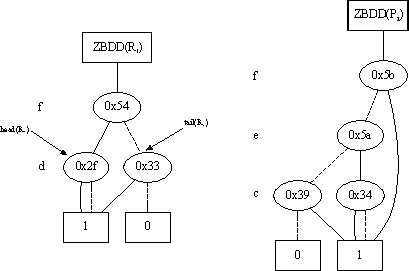
\includegraphics[scale=1]{r1_p1.pdf}
\caption{ZBDD for polynomial $R_1$ and $P_2$}
\label{P2}
\end{figure}


\par Next we will show how reduction can be performed using ZBDDs. In step 2, the polynomial, $P = fd +f +d $, needs to be reduced by $P_2$. The ZBDDs for $P$ and $P_2$ are shown in Figure~\ref{red_steps} and~\ref{P2} respectively. The ZBDD for $P$ has three paths ($fd,f,d$) terminating in the node 1 that correspond to its monomials. The ZBDD manager creates the ZBDDs with the defined monomial order, and therefore, the topmost node in both ZBDDs is $f$. %Checking if $lm(P_2)$ divides $lm(P)$ becomes trivial as we just need to compare the indices of top-most nodes of ZBDDs of $P$ and $P_2$, which in this case are equal. 

The algorithm for conventional reduction procedure using ZBDDs is shown in Algroithm~\ref{singlemon}. The procedure takes $F$ and $POLY\_LIST$ as input arguments. $F$ is the polynomial that we need to reduce $w.r.t.$ the polynomials (corresponding to the gates of the circuit),  $G \in POLY\_LIST$. The variables in the ZBDD manager are declared in the same order as the RTTO. For our example of Figure~\ref{ChainOrGate}, the first variable declared in the ZBDD manager is $z$, then $f$, and so on. If a circuit has polynomials, $P_1= x_1 + tail(P_1) \cdots P_d= x_d + tail(P_d)$ with variable order $x_1 > \cdots > x_d$, then the first element of the list, $POLY\_LIST$ is $P_1$, second $P_2$, and the last $P_d$. The top-most node in a ZBDD corresponds to the variable that has highest precedence in the RTTO. Populating $POLY\_LIST$ in this way avoids the search required to find a polynomial $G \in POLY\_LIST$ that can divide the leading term of $F$. While iterating over the polynomials $G \in POLY\_LIST$ if a certain polynomial does not divide the leading term of $F$, it will imply that polynomial is not in the logical cone of $F$.  

\par The procedure, $ leading\_term(G)$, takes in a ZBDD as an input argument and returns the leading term of the polynomial that the ZBDD represents. The procedure starts at the root node and follows the THEN path until it reaches the terminal node 1. The cube of the variables, whose corresponding nodes are encountered on this path, gives us the leading term of the polynomial. The procedure, $Cudd\_zddDivide(A,B)$, takes two ZBDDs as input argument where B can only be a cube. If $B$ divides $A$, it returns the quotient of the division,  else it returns zero.
\par The polynomial, $F$, is completely reduced $w.r.t.$ the polynomial $G$ in the while loop. The $\cdot$ operator computes the product of two ZDDs. Also, the + operator is a modulo 2 sum which can be implemented as,
\begin{center}
$A + B = A \cup B - A \cap B$, where $A$ and $B$ are two ZBDDs
\end{center}
$\cup$ and $\cap$ are set union and set intersection operations respectively. This computation results in large intermediate ZBDDs for the union of $A$ and $B$. Therefore, this operation and the product is implemented using the Recursive Boolean Addition and Product algorithm as presented in~\cite{polybori}. 

\begin{algorithm}
\caption{Single Monomial Reduction}
\label{singlemon}
\begin{algorithmic}[1]
\Procedure{$single\_mon\_red$}{$F,POLY\_LIST$}
\For{each $G \in POLY\_LIST$}
\State $lead\_G = leading\_term(G)$
\State $lead\_F = leading\_term(F)$
\State $divide = Cudd\_zddDivide(lead\_F,lead\_G)$
\While{$divide \neq zero$}
\State $prod = divide \cdot G$
\State $F = F + prod$
\State $lead\_F = leading\_term(F)$
\State $divide = Cudd\_zddDivide(lead\_F,lead\_G)$
\EndWhile
\EndFor
\State \Return F
\EndProcedure
\end{algorithmic}
\end{algorithm}
\par As the polynomial, $F$, changes for every iteration of the while loop, the ZBDDs in $lead\_F$ and $divide$ are updated everytime at the end of the loop. When $F$ no longer contains the leading term of a polynomial $G$ in any of its terms, the procedure $Cudd\_zddDivide$ returns zero and the while loop terminates. The total number of iterations of the nested loops for the example of Figure~\ref{ChainOrGate} is 7.
%\par The process repeats for all the polynomials $G \in  POLY\_LIST$. The procedure returns $F$, which has been completely reduced $w.r.t.$ the polynomials in the list $POLY\_LIST$. 

\begin{algorithm}
\caption{Multi-Term Reduction Algo 1}
\label{multimon}
\begin{algorithmic}[1]
\Procedure{$multi\_mon\_red\_1$}{$F,POLY\_LIST$}
\For{$i$ from $0,1,...,size(POLY\_LIST)-1$}
\State $G_i = POLY\_LIST[i]$
\State $index_{G_i} = G_i \rightarrow index$
\State $index_F = F \rightarrow index$

\If{ $index_{G_i} == index_f$} 
%\State $p_1 = then(f)$
%\State $p_2$ = else(f)
%\State tail = else($g_i$)
%\State prod = $p_1$ $ \cdot$  tail
\State $F = ELSE(F) + THEN(F)\cdot ELSE(G_i)$
\EndIf

\EndFor
\State \Return F
\EndProcedure
\end{algorithmic}
\end{algorithm}

\par Next, we will show how $P = fd + f + d$ can be reduced by $P_2$ in one step i.e eliminating the need of the while loop in Algorithm~\ref{singlemon}. If we check the THEN branch of node $f$ in $P$ (Figure~\ref{red_steps}), we will find that it represents the polynomial, $d + 1$. Therefore, the THEN branch of the top-most node of $F$ gives us all the terms that appear with $f$. So the reduction can be performed by multiplying $d + 1$ with $P_2$ and adding this product to $F$ $\pmod{2}$ ,
\begin{align*}
& (fd + f + c) + (d + 1)\cdot(f + ec + e + c) \pmod{2}\\
&= 2\cdot(fd + f) + c + (d+1)\cdot(ec + e + c) \pmod{2}\\
&= c + (d+1)\cdot(ec + e + c)  \pmod{2}
\end{align*}
Consider the follwing terminologies,
\begin{align*}
& \text{$head(F)$ = THEN branch of top-most node of $F$} = d + 1\\
& \text{$tail(F)$ = ELSE branch of top-most node of $F$} = c\\
& \text{$head(G)$ = THEN branch of top-most node of $G$} = f\\
& \text{$tail(G)$ = ELSE branch of top-most node of $G$} = ec + e + c
\end{align*}
In the above example, we know that $2\cdot(fd + f) \pmod{2}$ is going to be zero. Therefore, in order to reduce number of operations, we directly use the last step as a formula for reduction, $F \xrightarrow{G}_+$,
\begin{align*}
&= c + (d+1)\cdot(b + a) \\
& tail(F) + head(f)\cdot tail(G)
\end{align*}
The data structure for a ZBDD node has two pointers for the THEN child and ELSE child, respectively. Therefore, $head(F)$, $tail(F)$, and $tail(G)$ can be acquired by just accessing the respective pointers. So the reduction process effectively involves two operations, a modulo 2 sum and a product.

The algorithm for Multiple Monomial Reduction is shown in Algorithm~\ref{multimon}, where the notations, $F$ and $POLY\_LIST$, are same as that for the Single Monomial Reduction algorithm. Unlike in Algorithm~\ref{singlemon}, where we need to find the quotient of $lead\_F/lead\_G$, in Algorithm~\ref{multimon} we only need to determine if $lead\_G$ can divide $F$ at all (in this case the quotient is $THEN(F)$). This can be accomplished by just comparing the indices of top-most nodes of $F$ and $G$. This algorithm significantly cut down the number of iterations which are now equal to the size of $POLY\_LIST$ for each output. For the example Figure~\ref{ChainOrGate}, the number of iterations is 3 using Algorithm~\ref{multimon}.
%The name multi-term is due to the reason that $g_i$ reduces f by multiple terms in one iteration as opposed to single term(while loop in Single-Term Reduction Algorithm). 

The AND-XOR heuristic presented in~\cite{rolf:2016} can also be implemented on the ZBDD framework. $VAR\_LIST$ is the list of the variables in the polynomial model. We create another list, \textit{XVAR\_LIST}, that contain all the variables except the inputs and outputs variables of XOR gates and primary inputs and outputs in the circuits. While iterating over all the polynomials, $G_i$, in the \textit{POLY\_LIST}, we check if the ELSE part, $e$, of $G_i$ contain any variable from the \textit{XVAR\_LIST}. This can be done using the sub-routines for finding the support of a ZBDD and checking if any of these variables are contained in the \textit{XVAR\_LIST}. If it does, we reduce $e$ with the polynomial that has that variable as the leading term using a variant of Multi-Term Reduction algorithm, presented in Algorithm~\ref{multimon2}. This algorithm can reduce the ZBDD of a polynomial either by another polynomial or a cube depending on the value of the parameter, $par$. The polynomial $e$ is then reduced by the cube of pair of AND-XOR variables which have been already extrated from the circuit topology and stored in the list, $AX\_LIST$. Reducing a polynomial by a cube of type $x_i \cdot x_j$ is equivalent to replacing all the monomials containing this cube with zero. 
\par A similar algorithm for applying the fan-out heuristic is also implemented. The algorithm will take a list, instead of $XVAR\_LIST$, that contains all the variables except the the ones that occur in the $tail$ of more than one polynomial and primary inputs and outputs.

\begin{algorithm}
\caption{AND-XOR Elimination}
\label{and-xor}
\begin{algorithmic}[1]
\Procedure{\textit{and\_xor}}{\textit{POLY\_LIST,XVAR\_LIST}}
\For{$G_i \in POLY\_LIST$}
\State $e = ELSE(G_i)$
\State $s = SUPPORT(e)$
\For{\text{each} $var \in s$}
\If{$var \in XVAR\_LIST$}
\State $e = multi\_mon\_red\_2(e,POLY\_LIST[var \rightarrow index],0)$
\For{\text{each} $p \in AX\_LIST$}
\State $e = multi\_mon\_red\_2(e,p,1)$
\EndFor
\EndIf
\EndFor
\State $G_i = ITE(VARS(i),THEN(G_i),e)$
\EndFor
\EndProcedure
\end{algorithmic}
\end{algorithm}

\begin{algorithm}
\caption{Multi-Term Reduction Algo 2}
\label{multimon2}
\begin{algorithmic}[1]
\Procedure{$multi\_mon\_red\_2$}{$G_i,R,par$}
\If{$par == 0$}
\State $divide = Cudd\_zddDivide(G_i,VAR\_LIST[R \rightarrow index])$
\Else
\State $divide = Cudd\_zddDivide(G_i,R)$
\EndIf

\If{$divide \neq 0$}
\State \Return $F + G_i\cdot divide$
\Else
\State \Return $F$
\EndIf


\EndProcedure
\end{algorithmic}
\end{algorithm}

%Let f = $ab + a + b + c$ and $g_i$ = $a + de$ and the variable order $a > b > c > d > e$. The corresponding ZDDs are shown below: \par
%%Insert figure%%%%%%%%%%%%%%%%%%%%%%%%%
%Note that the topmost level in the ZDD is always composed of the variable with the highest precedence in the corresponding polynomial. The ZDD manager assigns an unique index number for each variable defined. Since the variables f and $g_i$ have the reference to the topmost node of the polynomial in f and $g_i$ (which is $a$ for this example), $g_i$\_index and f\_index have the index nuimber for the topmost node in the respective ZDDs. Next, we check if the index number are same or not(if same, it means $g_i$ can divide f; if not, otherwise). If the indices are same, $p_1$($p_2$) is assigned the ZDD connected to the "then"("else") branch of topmost node of f. From the figure, the ZDD connected to "then"("else") branch of $a$(which is the topmost node) is the polynomial $b + 1$ ($b + c$). Evaluating the sum (modulo 2) of f($ab + a + b + c$) and $p_1$ $\cdot$ $g_i$( ($b + 1$)$\cdot$($a + de$) ) will result in a polynomial that corresponds to f being completely reduced with respect to $g_i$. The terms in f containing $a$ will get cancelled by the terms ($b + 1$)$\cdot$($a$) in the product $p_1$ $\cdot$ $g_i$. Inorder to minimize computations, the algorithm finds f by just adding the $p_2$ (terms not containing $a$ in f) and prod, which is the product of $p_1$ and the part of $g_i$ free of variable $a$. The process is repeated for every $g_i$ in G. The procedure returns f, which is only composed of primary inputs.
\bibliography{refer}


\end{document} 